\documentclass[USenglish,oneside,twocolumn]{article}

\usepackage[utf8]{inputenc}%(only for the pdftex engine)
%\RequirePackage[no-math]{fontspec}%(only for the luatex or the xetex engine)
\usepackage[big]{dgruyter_NEW}

\DOI{foobar}

\cclogo{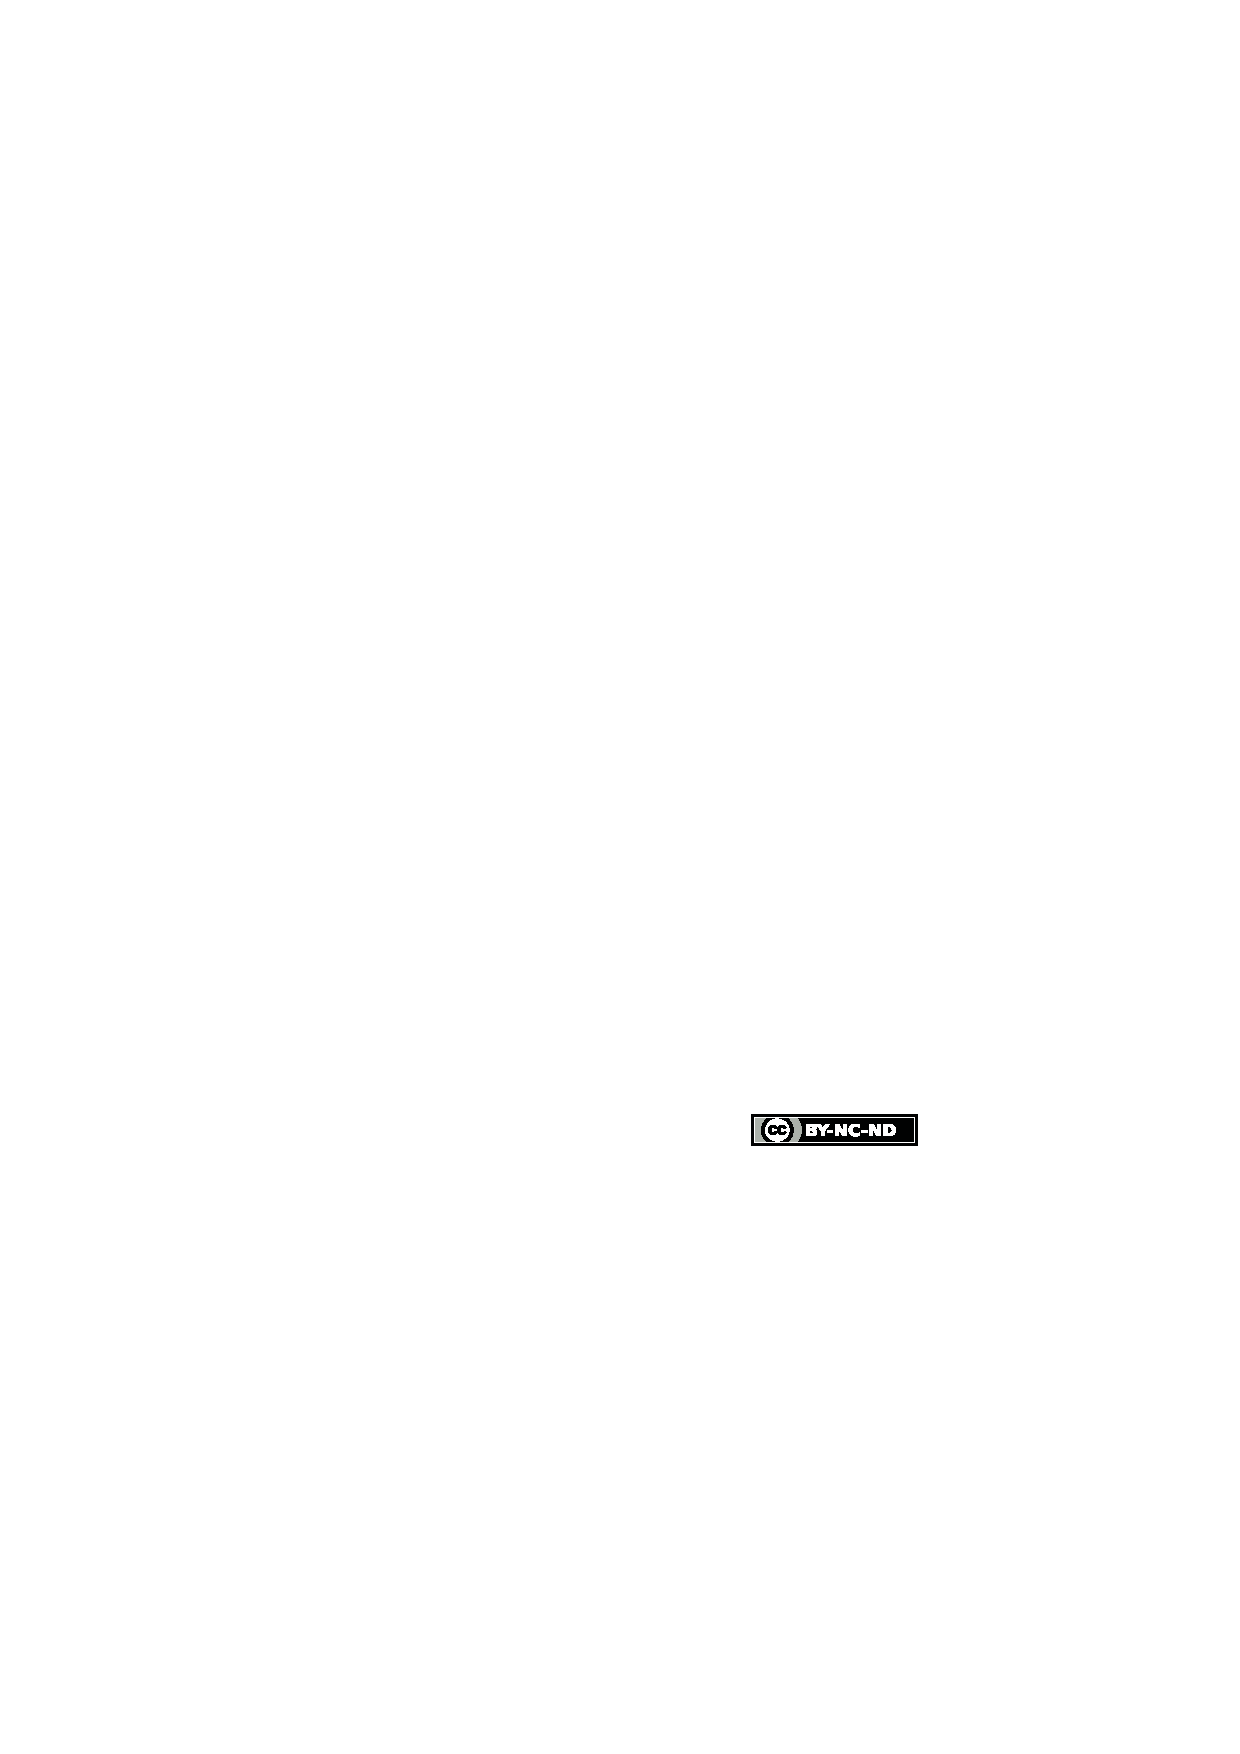
\includegraphics{by-nc-nd.pdf}}

% Related work comparison table
\usepackage{amsmath,wasysym} % \CIRCLE, \Circle
\usepackage{multirow} % \multirow
\usepackage{times} % font in table header


\begin{document}


  \author[1]{Anthony P. Machado}

  \author[2]{Gaby G. Dagher}

  \author[3]{Eddie C. Davis}

  \affil[1]{Boise State University, E-mail: anthonymachado@u.boisestate.edu}

  \affil[2]{Boise State University, E-mail: gabydagher@boisestate.edu}

  \title{\huge Hiding Data in Cellular DNA: Contextualizing Diverse Encoding Schemes}

  \runningtitle{Hiding Data in Cellular DNA}

  \providecommand{\e}[1]{\ensuremath{\times 10^{#1}}}

  %\subtitle{...}

  \begin{abstract}
{DNA, the macromolecule used by organisms to store and transmit genomic data, has attracted the attention of privacy researchers as a channel for secure data transfer. DNA's small size and abundance in nature makes it an ideal steganographic medium for hiding messages. Already, artificially synthesized DNA has been used to store text, audio, and images. Encoded cellular DNA is not far behind, with much research being done on ways to safely embed data without harming the cell. \\
In this survey we provide the first systematic comparison of cellular encoding schemes proposed in the literature. Different DNA regions in the cell have their own unique bio-restrictions that must be satisfied for DNA storage. Drawing from a wide array of schemes, we compare the novel techniques used to meet these bio-restrictions. This contextualization of the research creates a bigger picture that can help guide the design of future schemes. We also survey the compression methods and error detection techniques used by the encoding schemes, and their effect on error rate and bits-per-base density. Finally, we propose future directions for research in untapped cellular regions such as mitochondrial DNA and we offer novel insights into the potential for epigenetic encoding with methylation and histones.}
\end{abstract}

  \keywords{keywords, keywords}
%  \classification[PACS]{}
 % \communicated{...}
 % \dedication{...}
 % \test

  \journalname{Proceedings on Privacy Enhancing Technologies}
\DOI{Editor to enter DOI}
  \startpage{1}
  \received{..}
  \revised{..}
  \accepted{..}

  \journalyear{2017}
  \journalvolume{2017}
  \journalissue{3}


\maketitle
\section{Introduction}

Biosteganography is an emerging field in privacy research that combines techniques from genetic engineering, bioinformatics, cryptography and forensics to secretly transfer data within a living cell's DNA~\cite{B2016JOB}. Data ranging from simple text messages to audio recordings and color images can be inserted into cellular DNA for secure transmission. Because DNA is information dense and occurs abundantly in nature, it makes an ideal medium for sending messages secretly. Basic steganographic principles dictate that if an attacker doesn’t know where to find a confidential message in the first place, the message is far more secure~\cite{A2001IEEEIC}. Locating encoded DNA would be harder than finding a needle in a haystack. A needle, at least, can be seen by the human eye.

Traditional digital storage systems such as hard drives and SD cards have detectable emanations, which makes them vulnerable to side attacks~\cite{T2008TOIAS}. Modified DNA, however, has no measurable emanations. If an agent needed to carry a confidential message through a tight security checkpoint, any form of electronic storage could be easily detected, while physical recordings like paper or tape could be visibly located by the security guard. A DNA encoded message, however, located in the cells of the agent's thumb, or in bacteria under the agent's nail, could be brought through without detection. The receiver of the message would need to know how to decode the data, and have the lab equipment to amplify and sequence the DNA in order to retrieve the message.

Inserting hidden data into DNA is also crucial for watermarking patented genes. Advances in gene editing technology have led to a rise in genetically modified organisms being developed in a variety of sectors such as agriculture, healthcare, and energy. For added security of these novel genomes, many companies have begun embedding hidden watermarks in their DNA so that ownership can be established in the case of theft. For this purpose too, secrecy is essential. The watermark must be embedded in such a way that the thief cannot find it, else the thief would simply remove it. Thus, biosteganography is an overlapping goal both of individuals wanting to send data privately and companies wanting to watermark genetic inventions.

Many encoding schemes have been proposed to accomplish data embedding in cellular DNA.

In this survey, we will provide the first systematic analysis of these diverse encoding schemes, in which:
\\
\begin{itemize}
\item we define the unique bio-restrictions associated with cellular encoding and compare how the proposed encoding schemes meet these restrictions;
\item we contrast the error rates and bits-per-nucleotide densities of each of the schemes, highlighting the effects of error correction and compression techniques on both; and
\item we propose new directions for research incorporating novel epigenetic techniques.
\end{itemize}

The rest of the survey is organized as follows. In Section 2 we provide a background on genetics, explain techniques in artificial DNA encoding, and clarify the biological restrictions involved in cellular encoding. A systematic comparison of the encoding schemes for coding and non-coding regions is presented in Section 3, in which we look at how each encoding scheme meets cellular restrictions and the error rate and bits-per-nucleotide density it offers. Finally, in Section we propose new directions for future encoding schemes that use epigenetics and alternative genetic regions.


\section{Background}

\subsection{DNA}

Every living cell contains DNA molecules encoded with instructions for making the proteins necessary for the cell to function. DNA takes the form of a double helix made of two antiparallel strands. Each strand is composed of a sequence of 4 nucleotides: adenine (A), guanine (G), cytosine (C), and thymine (T). The purines adenine and guanine, and the pyrimidines cytosine and thymine, form hydrogen bonds with each other across the double helix. Adenine binds to thymine with two H-bonds, and guanine binds to cytosine with three. Every three nucleotides forms a codon that the cell reads and processes to create an amino acid, the building block of a protein~\cite{WC1953N}. Proteins can be encoded on either strand.

There are only 20 amino acids, despite the fact that $4^3$ = 64 possible codon variations exist. This is because many amino acids are correlated with up to five redundant codons. Also, three codons are used specifically as stop signals to indicate the end of a protein chain. The redundancy in codon to amino acid mapping is called codon degeneracy~\cite{WBBGLL2008}. Codon degeneracy gives an evolutionary advantage to the cell by allowing certain mutations to occur in a codon while preserving the codon’s functionality.

\begin{center}
 \scalebox{.85}{
 \begin{tabular}{||c || c c c c c c||}
 \hline
 Amino & & & Codons & & &\\ [0.5ex]
 Acids & & & & & &\\ [0.5ex]
 \hline\hline
 Ala & GCT & GCC & GCA & GCG & &\\
 \hline
 Arg & CGT & CGC & CGA & CGG & AGA & AGG \\
 \hline
 Asn & AAT & AAC & & & &\\
 \hline
 Asp & GAT & GAC & & & &\\
 \hline
 Cys & TGT & TGC & & & &\\
 \hline
 Gln & CAA & CAG & & & &\\
 \hline
 Glu & GAA & GAG & & & &\\
 \hline
 Gly & GGT & GGC & GGA & GGG & &\\
 \hline
 His & CAT & CAC & & & &\\
 \hline
 Ile & ATT & ATC & ATA & & &\\
 \hline
 Leu & TTA & TTG & CTT & CTC & CTA & CTG \\
 \hline
 Lys & AAA & AAG & & & &\\
 \hline
 Met & ATG & & & & &\\
 \hline
 Phe & TTT & TTC & & & &\\
 \hline
 Pro & CCT & CCC & CCA & CCG & &\\
 \hline
 Ser & TCT & TCC & TCA & TCG & AGT & AGC \\
 \hline
 Thr & ACT & ACC & ACA & ACG & &\\
 \hline
 Trp & TGG & & & & &\\
 \hline
 Tyr & TAT & TAC & & & &\\
 \hline
 Val & GTT & GTC & GTA & GTG & &\\
 \hline
 START & ATG & & & & &\\
 \hline
 STOP & TAA & TGA & TAG & & &\\[1ex]
 \hline
\end{tabular}}
\end{center}

\subsection{Artificial Encoding}

Artificial DNA encoding, or DNA data storage, is the process of storing digital information such as text, audio, or images within \textit{in vitro} DNA base pair sequences. DNA is an appealing storage medium due to its high density. For example, the human genome contains 3.3\e{9} base pairs, or about 725 MB of binary data, with a mass of 3.59\e{-12} grams. DNA is also incredibly resilient, as the sequencing of 45,000 year old woolly mammoth genomes indicate~\cite{PALKOPOULOU2015}. As with any memory device, the critical operations are read and write. Continued advances in DNA sequencing (reading) and oligonucleotide synthesis (writing) increase the viability of nucleic acid for long term archival storage.

DNA was first encoded with a secret message in 1999 by Clelland et al~\cite{CRB1999N}. Inspired by the tiny, concealed “microdot” messages used in World War II, artificial DNA strands were constructed using a simple substitution cipher, then mixed with human DNA and pipetted onto a printed period on filter paper. The encoded DNA was later recovered from the dot and sequenced to successfully read the secret message: “JUNE 6 INVASION: NORMANDY”.

The primary limiting factor has been the length of the oligonucleotides that can be synthesized. Church et al.~\cite{CHURCH2012} developed a technique using high fidelity DNA microchips to encode 5.27 MB of data including a book by the author, 11 JPEG images, and a JavaScript program into 54,898 159 nt sequences. Each 159 nt sequence consisted of a 96 nt data block and 19 nt address. The data were recovered with only 10 bit errors.

Goldman et al.~\cite{GOLDMAN2013} were able to encode 739 KB of text, images, and audio with 100\% recovery rate. The technique applied a modified Huffman code~\cite{H1952POTIRE}, converting the binary (base-2) data into ternary (base-3), and mapping each trit to a nucleotide, different from the one preceding it in order to prevent homopolymers. The sequences were capped with reverse complemented index information so that the data could be reassembled by scanning for overlaps.

Grass et al.~\cite{GRASS2015} developed error correction codes for DNA stored in silica gel and exposed to high temperature ($70^o$ C).

Yazdi et al.~\cite{YAZDI2015} also developed some sort of DNA error correction code, but I have not yet read trough the paper.

Blawat et al.~\cite{BLAWAT2016} improved upon this work by developing forward error correction codes.

\subsection{Cellular Encoding Restrictions}

Cellular DNA encoding must not harm the carrier organism, either by removing cellular functionality or adding mutative behavior. To avoid this, encoding schemes must ensure that modified DNA strands remain biologically equivalent to their wild-type form. This section defines the bio-restrictions that exist for two distinct areas of cellular DNA, protein coding DNA (pcDNA) and noncoding DNA (ncDNA). As our knowledge of genetics continues to expand, more particular restrictions may become known.

\subsubsection{pcDNA Constraints}

The protein coding region of DNA contains the codons that are translated to amino acids, which are concatenated into proteins. Any data insertions in this area must meet the following constraints.

\textit{Protein Preservation} The structure of the protein coded by the region must remain unchanged. Nucleotide insertions and modifications must not alter the codons in such a way that would change the original amino acid sequence.

\textit{Codon Bias Preservation} Individual cells have specific ratios of cytoplasmic tRNA associated with their genomic codons, which can be disrupted if the codon balance is changed, and have a negative effect on the cell. Therefore, it is important that codon bias is preserved.


\subsubsection{ncDNA Constraints}

The noncoding region of DNA is often called "junk DNA" for its apparent lack of use in the cell. Because they appear to be non-functional, data can be embedded into these regions if the following constraints are met.

\textit{Truly nonfunctional region.} When ncDNA was first discovered it was assumed to have no role in cell functionality, but recent studies have shown that up to 80\% of ncDNA may have biochemical functions in the cell, despite not coding for proteins~\cite{EPC2012N}. Therefore, it is first imperative that the individual who wishes to insert a message into ncDNA verify that they are encoding their message in the 20\% that has no biochemical use.

\textit{No start codons.} When a cell's genetic machinery locates a start codon, it can begin the transcription process. To prevent unwanted transcription from happening in ncDNA with embedded data, it is important to make sure the encoded nucleotides to not create a start codon. When a DNA string is being transcribed, three-nucleotide codons can be read in six different reading frames. Therefore, there should not be a start codon in any of the six frames. The most common start codon is AUG, though some alternative start codons can also exist, particularly in bacteria~\cite{B1997S}. If a cell contains alternative start codons, the encoding scheme should avoid all of them.

\textit{No homopolymers.} A DNA homopolymer is a region where the same nucleotide is repeated multiple times. Too many repeats can cause errors during DNA replication through polymerase slippage~\cite{VCE2001TEJ}. These replication errors could quickly distort the inserted message and possibly damage the cell after a few generations. For this reason any ncDNA encoding scheme should not include homopolymers greater than length 3.

\section{Compression and Error Correction}

Smith et al.~\cite{SFHC2003BL} were the first to suggest a data compression technique in DNA encoding, specifically the Huffman Code. The Huffman Code is a form of lossless data compression that forms a symbol table using fewer bits to encode more common characters~\cite{H1952POTIRE}. Smith et al created a Huffman Code table mapping letters of the alphabet to nucleotide strings, where the most common English letter 'e' was mapped to the nucleotide string "T", and the least common english letter 'z' was mapped to a longer nucleotide string "CCCTG". This achieved an average encoding length of 2.2 bases per letter. The mapping is unambiguous, making only one possible interpretation of each message.

Comma encoding~\cite{BVSPNAS2000} specifies that encoded words be separated by a single nucleotide (i.e., G). The remaining four (or five in Smith et al.), are composed of the other three nucleotides. Additional constraints are that only three A-T pairs are allowed, and two G-C always on the top strand, so that the DNA molecules will have isothermal melting temperatures. This technique provides particularly good detection of insertions and deletions, unfortunately it is also space inefficient.

The alternating code, also from Smith et al.~\cite{SFHC2003BL} consists of 64, 6 base pair codons, with nucleotides alternating between an A or G (purines) at odd positions, and C or T (pyrimidines) at evens (e.g., RYRYRY…, YRYRYR). Like the comma encoding, the alternating code results in isothermically stable molecules with a 1:1 ratio of A-T to G-C pairs. While more space efficient, this technique is not as proficient at error detection, as only 67\% of codons result in nonsense codons after mutation, compared to 83\% for the comma code.

Contrast mapping is an encoding scheme developed by Mousa et al.~\cite{MMAIAJI2011}. The binary message is divided into 6-bit groups, each converted to decimal (base 10). Pairs of consecutive values ($x, y$) are converted into ($x', y'$) with the the following linear transformations: $x' = 2x - y$,  $y' = 2y - x$. Values are limited to the subdomain:  0 $\leq$ 2$x - y$ $\leq$ $L$, 0 $\leq$ 2$y$ - $x$ $\leq$ $L$. Values are decoded with the following equations: $x = [3x' + 3y'], y = [3 x' + 3y']$. This technique is sufficiently flexible to be applied to DNA or image steganography.

\section{Encoding Schemes}

Encoding schemes for cellular DNA can involve several components:

\begin{enumerate}
\item Encryption algorithm
\item Mapping table
\item Compression
\item Error correction
\item Fake data embedding
\end{enumerate}

The following encoding schemes use some or all of these elements in their design.



\subsection{pcDNA Encoding}

Shimanovsky et al~\cite{SFHC2003BL} were the first to propose using codon degeneracy to encode data in pcDNA. By switching codons between their redundant forms with the modification of one nucleotide, data was inserted without altering protein translation. Arita and Ohashi~\cite{AY2004BP} implemented this technique in a living cell. They did this using site-directed mutagenesis of wobble codons in the \textit{ftsZ} gene of \textit{Bacillus subtilis}. The university name "KEIO" was inserted by modifying the redundant nucleotides of the codons downstream of the \textit{ftsZ} start codon. An unmodified codon represented value 0 while a codon with a wobble nucleotide changed to any of its non-wild type redundant forms represented value 1. Messages were translated using a 6-bit mapping table, with the first 5 bits corresponding to an English alphabet letter or basic punctuation, and the last used as a parity bit for error correction.

Heider et al. developed the DNA-Crypt~\cite{HBBMC2007} algorithm for creating DNA watermarks for marking genetically modified organisms. It is similar to the work of Arita et al. in that the encoding targets the wobble base pair in the genetic code. An encryption function $E$ maps the plaintext (binary data) $X$ to the ciphertext (genetic data) $Y$, such that $X \in  \{$0, 1$\}$ and $Y \in \{$A, C, G, T$\}$. Two bits are encoded per base, or one byte for four bases. Error correction is achieved with a fuzzy controller that selects one of two algorithms, either the 8/4 Hamming code for mutations that differ in only bit (e.g., 00 to 01) or the WDH-code for those that differ by multiple bits. This encoding scheme allowed implementations of several cryptographic algorithms, including One-Time Pad, AES, Blowfish, and RSA. The accuracy was tested using the GTPase encoding Ypt gene in $S. cerevisiae$.

Haughton and Balado proposed BioCode~\cite{HBBMC2013}, a pair of encoding algorithms, one for ncDNA, and one for pcDNA. The ncDNA algorithm expands upon DNA-Crypt by observing the no start codons in restriction. This is accomplished by defining a set of dinucleotides $D$ = $\{$ AT, CT, TT, CA $\}$ that covers the possible eukaryotic start codons on either DNA strand. The trailing dinucleotide $d$ is continually checked for membership in $D$. If found, $d$ is replaced with a lookup table formed from a graduated mapping of the message space $M_d$ to set $S_d$. The pcDNA encoding technique is similar, but enforces the additional constraint of Binary Codon Equivalency (BCE). This requires that the cardinality of the codon set (|$S_d$|) be varied during the embedding process to allow the usage of a static lookup table.

In order to better preserve codon bias, Lee developed a discrete wavelet transform (DWT) technique for pcDNA encoding~\cite{L2014IS}. The target coding sequence was divided into subsequences in which every codon was given a numerical code associated with amino acid histogram rankings. DWT coefficients were calculated for synonymous codons and the optimal subsequence was found, which was then replaced with the encoded subsequence. A nonlinear congruential-pseudorandom number generator then created the watermark and picked the location in the DWT domain for embedding.

\subsection{ncDNA and Plasmid Encoding}

The development of encoding schemes for ncDNA and plasmids have been strongly correlated, due to two regions having nearly identical bio-restrictions. The main difference being that plasmid encoding is also confined by length. However, due to their similarities and the parallel advancement of their encoding schemes, we will consider them both in this section.

Wong et al.~\cite{WWF2003COTACM} were the first to encode data into plasmids. Letters and punctuation were mapped to nucleotide triplets, then short text snippets of 19 to 33 characters were inserted into the plasmids of Deinococcus radiodurans, a bacteria that is very resilient to extreme conditions. The encoded section of the plasmid was flanked by sentinel sequences 20 base pairs long containing stop codons. This was done to prevent the bacteria from transcribing the message while reading the adjacent functional parts of the plasmid. After insertion of the plasmids into the host bacteria, they were incorporated into their genomes. No error correction, encryption, or compression techniques were used.

Yachie et al.~\cite{YSSOT2007BP} came up with the idea of using multiple alignment in lieu of error detection or correction techniques. With this scheme, messages were composed using the Keyboard Scan Code Set2, which contains all keyboard inputs, and converted these messages to binary. The encryption keys mapped four bits of binary code to two nucleotides. This type of mapping created four reading frames in the binary message (C1 - C4), each of which was converted to DNA and inserted adjacently into the plasmid, creating redundancy that allowed for multiple alignment when decoding.

Repetition coding was used again, this time for ncdDNA, by Haughton and Balado ~\cite{HB2011IEEEICOBAB} who used two variant approaches. Both approaches required finding subsequences in the host ncDNA equal to the length of the encoded message, and replacing them with the message, as opposed to simply inserting the message and expanding the DNA strand. With the first approach, $RAlign$, the redundant subsequences were each prepended and appended with unique 24-bp long markers to aid alignment, and replaced specific subsequences in the genome that were known by both the sender and receiver. With the second approach, $HTAlign$, the prepended and appended markers were identical, which means the receiver does not need to know the location of the replaced subsequences, but can find the repeated messages by searching for the markers alone.

Wanting to improve on the very low bits per base density of previous schemes, Ailenberg and Rotstein suggested an improved Huffman code that could decrease the sequence sizes by up to 40\%~\cite{AR2009BT} compared to other schemes. Keyboard characters were mapped to variable length sequences, with the more common characters assigned to the shorter sequences. To help maintain C-G balance, CG-rich codons were pushed downwards on the frequency table. To illustrate the density that could be achieved, text and musical notes for "Mary Had a Little Lamb", along with an image of a lamb made with geometric shapes, were encoded into a mere 844-bp DNA fragment. It was estimated that this encoding scheme would average 3.5 bases-per-character, which was a noted improvement over previous schemes. No error correction was used.

\begin{table}[h]
	\caption{Table 1}
	\label{fig:table1}
	\centering
	\scalebox{0.6}{
	\begin{tabular}{|c|c|c|c|c|c|c|c|c|c|c|}\hline \hline
		Method  &  &  &Bio-Restrictions  &  &  &Error Detection  &Error Correction  &Compression  &Encryption  &Blind Decoding\\ \hline
		  &No Homopolymers  &No Start Codons  &Preserves Functionality  &Preserves Codon Bias  &Balances C-G  &  &  &  &  &\\ \hline
		PROTEIN CODING DNA  &  &  &  &  &  &  &  &  &  &\\ \hline
	Secret Signature~\cite{AY2004BP}  &\centering{$\CIRCLE$}  &\centering{$\CIRCLE$}  &\centering{$\CIRCLE$}  &  &  &\centering{$\CIRCLE$}  &  &  &  &\\ \hline
		DNA-Crypt~\cite{HBBMC2007}  &\centering{$\CIRCLE$}  &\centering{$\CIRCLE$}  &\centering{$\CIRCLE$}  &  &  &\centering{$\CIRCLE$}  &\centering{$\CIRCLE$}  &  &\centering{$\CIRCLE$}  &\\ \hline
		BioCode~\cite{HBBMC2013}  &\centering{$\CIRCLE$}  &\centering{$\CIRCLE$}  &\centering{$\CIRCLE$}  &\centering{$\CIRCLE$}  &\centering{$\CIRCLE$}  &\centering{$\CIRCLE$}  &\centering{$\CIRCLE$}  &  &  &\\ \hline
		DWT Based~\cite{L2014IS}  &\centering{$\CIRCLE$}  &\centering{$\CIRCLE$}  &\centering{$\CIRCLE$}  &\centering{$\CIRCLE$}  &\centering{$\CIRCLE$}  &\centering{$\CIRCLE$}  &\centering{$\CIRCLE$}  &  &  &\\ \hline
		  &  &  &  &  &  &  &  &  &  &\\ \hline
		NONCODING DNA and PLASMIDS  &  &  &  &  &  &  &  &  &  &\\ \hline
        Organic Memory~\cite{WWF2003COTACM}  &  &  &\centering{$\CIRCLE$}  &\centering{$\CIRCLE$}  &  &  &  &  &  &\\ \hline
		Alignment-Based~\cite{YSSOT2007BP}  &  &  &\centering{$\CIRCLE$}  &\centering{$\CIRCLE$}  &  &\centering{$\Circle$}  &\centering{$\Circle$}  &  &  &\\ \hline
		Improved Huffman~\cite{AR2009BT}  &  &  &\centering{$\CIRCLE$}  &\centering{$\CIRCLE$}  &\centering{$\Circle$}  &  &  &\centering{$\CIRCLE$}  &  &\\ \hline
		Regulatory Watermarks~\cite{HPB2009BMCRN}  &  &  &  &  &  &  &  &  &  &\\ \hline
		RAlign~\cite{HB2011IEEEICOBAB}  &  &  &\centering{$\CIRCLE$}  &\centering{$\CIRCLE$}  &  &\centering{$\Circle$}  &\centering{$\Circle$}  &  &  &\\ \hline
		HTAlign~\cite{HB2011IEEEICOBAB}  &  &  &\centering{$\CIRCLE$}  &\centering{$\CIRCLE$}  &  &\centering{$\Circle$}  &\centering{$\Circle$}  &  &  &\\ \hline
		DNA Barcodes~\cite{KS2015BMCB}  &\centering{$\CIRCLE$}  &  &\centering{$\CIRCLE$}  &\centering{$\CIRCLE$}  &  &\centering{$\CIRCLE$}  &\centering{$\CIRCLE$}  &  &  &\\ \hline
		DNA-Courier Attack~\cite{CLY2015SAPW}  &  &  &\centering{$\CIRCLE$}  &\centering{$\CIRCLE$}  &\centering{$\CIRCLE$}  &  &  &  &\centering{$\CIRCLE$}  &\\ \hline
	\end{tabular}}
\end{table}

Heider et al.~\cite{HPB2009BMCRN} were interested in the possibility of encoding data in non-protein coding but biochemically functional DNA. 2-3 character watermarks were inserted into non-coding promoter regions and a regulatory RNA region in $Escherichia coli$. The introduction of the watermarks were shown to disrupt the reading of the genes associated with the promoters and changed the secondary structure of the regulatory RNA molecule. This research was significant in showing that biochemically functional ncDNA is a poor region for encoding.




\begin{table}[h]
	\caption{Comparative evaluation of encoding schemes}
	\label{fig:encoding_table}
	\centering
	\begin{tabular}{|c|c|c|c|c|c|c|c|c|c|}\hline \hline
		.  &Method  &Organism  &Bio-Restrictions*  &Error Correction  &Error Rate  &Compression Technique  &Bits/Base Density  &Blind Decoding  &etc?\\ \hline
		&  &  &  &  &  &  &  &  &\\ \hline
		Protein Coding DNA  &  &  &  &  &  &  &  &  &\\ \hline
		Kalifa, 2015  &LSBase  &  &H,S,F,C,G  &  &  &  &  &  &\\ \hline
		…  &  &  &  &  &  &  &  &  &\\ \hline
		Noncoding DNA  &  &  &  &  &  &  &  &  &\\ \hline
		Shimanovsky, 2002  &Codon redundancy  &  &F,C,G  &  &  &  &  &  &\\ \hline
		…  &  &  &  &  &  &  &  &  &\\ \hline
		Plasmids  &DNA Courier Attack  &  &H,S,F,C,G  &  &  &  &  &  &\\ \hline
		…  &  &  &  &  &  &  &  &  &\\ \hline
	\end{tabular}
\end{table}

There are several other regions of DNA that have seen little research in biosteganography, but have substantial potential for message encoding and watermarking.

\subsection{Mitochondrial DNA}

Heider et al.~\cite{HKB2008B} suggested using mitochondria for secret data encoding. Mitochondria are organelles in the cell that contain a small amount of DNA that encodes translation machinery and oxidative chain components~\cite{GV2001G}. Heider et al. identified an mtDNA section 1,541 base pairs long that contains no active gene regions and suggested that it would be an ideal location for embedding data with synonymous codons. They created a program called $Project Mito$, derived from $DNA-Crypt$, that encrypts binary files and modifies them with the Hamming code for error correction, before translating the message into an mtDNA sequence. $Project Mito$ can also be used for decryption after the DNA is sequenced.

\section{Conclusions}

\bibliographystyle{IEEEtran}
\bibliography{References}




\begin{table*}[!t]
    \centering
    \caption{Comparative evaluation of encoding schemes}
    \label{tbl:related_work}
    \scalebox{0.7}{
        \begin{tabular}{|p{5.7cm}|p{1.0cm}|p{0.7cm}|p{1.4cm}|p{1.1cm}|p{1.4cm}|p{1.1cm}|p{0.7cm}|p{0.8cm}|p{0.6cm}|p{0.8cm}|p{0.6cm}|p{1.1cm}|p{1.5cm}|}
            \hline
            \multirow{2}{*}{\vspace{-2cm}\textbf{Approach}} & \multicolumn{2}{|c|}{\textbf{Data Type}} & \multicolumn{4}{|c|}{\vspace{0cm}\textbf{Privacy-Preserving Domain}} & \multicolumn{5}{|c|}{\textbf{Hosting Environment}} & \multicolumn{2}{|c|}{\textbf{Security}} \tabularnewline
             \cline{2-14}
             & \vspace{0cm}\textbf{Set-Valued} & \vspace{0cm}\textbf{Other} & \multicolumn{2}{|c|}{\vspace{-.2cm}\textbf{Non-Interactive}} & \multicolumn{2}{|c|}{\vspace{0cm}\textbf{Interactive}} & \vspace{0cm}\textbf{Single} & \multicolumn{2}{|c|}{\vspace{-0.2cm}\textbf{Two}}& \multicolumn{2}{|c|}{\vspace{0cm}\textbf{Multiple}} & \vspace{0cm}\textbf{Threat Model $^\dagger$} & \vspace{0cm}\textbf{Public \newline Verifiability} \tabularnewline
             \cline{4-7}
             \cline{9-12}
             &  &  & \vspace{0cm}\textbf{Differential Privacy} & \vspace{0cm}\textbf{Syntactic Privacy} & \vspace{0cm}\textbf{Differential Privacy} & \vspace{0cm}\textbf{Syntactic Privacy}&  & \vspace{0cm}\textbf{Horiz.} & \vspace{0cm}\textbf{Vert.} & \vspace{0cm}\textbf{Horiz.} & \vspace{0cm}\textbf{Vert.}  &  & \tabularnewline
            \cline{1-14}
            \hline\hline
            Terrovitis \emph{et al.}, He and Naughton  & \centering{$\CIRCLE$} &  &  & \centering{$\CIRCLE$} &  &  & \centering{$\CIRCLE$} &  &  &  &  &  &  \tabularnewline
            \hline
            Chen \emph{et al.} &  \centering{$\CIRCLE$} &  &  \centering{$\CIRCLE$} &  &  &  & \centering{$\CIRCLE$} &  &  &  &  &  &  \tabularnewline
            \hline
            Jiang and Clifton &  &  \centering{$\CIRCLE$} &  & \centering{$\CIRCLE$} &  &  &  &  & \centering{$\CIRCLE$} &  &  & \centering{$\Circle$} &  \tabularnewline
            \hline
            Jurczyk and Xiong &  &  \centering{$\CIRCLE$} &  & \centering{$\CIRCLE$} &  &  &  &  &  & \centering{$\CIRCLE$} &  & \centering{$\Circle$} &  \tabularnewline
            \hline
            Alhadidi \emph{et al.} &  &  \centering{$\CIRCLE$} & \centering{$\CIRCLE$} &  &  &  &  & \centering{$\CIRCLE$} &  &  &  & \centering{$\Circle$} &  \tabularnewline
            \hline
            Mohammed \emph{et al.} (DistDiffGen) &  & \centering{$\CIRCLE$} & \centering{$\CIRCLE$} &  &  &  &  &  & \centering{$\CIRCLE$} &  &  & \centering{$\Circle$} &  \tabularnewline
            \hline
            Mohammed \emph{et al.} (TIPS) &  & \centering{$\CIRCLE$} &  & \centering{$\CIRCLE$} &  &  &  &  & \centering{$\CIRCLE$} &  &  & \centering{$\CIRCLE$} &  \tabularnewline
            \hline
            Bhaskar \emph{et al.}, Li \emph{et al.} & \centering{$\CIRCLE$} &  &  &  & \centering{$\CIRCLE$} &  & \centering{$\CIRCLE$} &  &  &  &  &  &  \tabularnewline
            \hline
            Wong \emph{et al.}  & \centering{$\CIRCLE$} &  &  &  &  &  & \centering{$\CIRCLE$} &  &  &  &  & \centering{$\Circle$} &  \tabularnewline
            \hline
            Giannotti \emph{et al.} & \centering{$\CIRCLE$} &  &  &  &  & \centering{$\CIRCLE$} & \centering{$\CIRCLE$} &  &  &  &  & \centering{$\Circle$} &  \tabularnewline
            \hline
            Kantarcioglu and Clifton & \centering{$\CIRCLE$} &  &  &  &  &  &  &  &  & \centering{$\CIRCLE$} &  & \centering{$\Circle$} &  \tabularnewline
            \hline
            Zhang \emph{et al.} & \centering{$\CIRCLE$} &  &  &  &  &  &  & \centering{$\CIRCLE$} &  &  &  & \centering{$\Circle$} &  \tabularnewline
            \hline
            Wahab \emph{et al.} & \centering{$\CIRCLE$} &  &  &  & \centering{$\CIRCLE$} &  &  & \centering{$\CIRCLE$} &  & \centering{$\CIRCLE$} &  & \centering{$\Circle$} &  \tabularnewline
            \hline
            Dwork \emph{et al.} &  & \centering{$\CIRCLE$} &  &  & \centering{$\CIRCLE$} &  &  &  &  & \centering{$\CIRCLE$} &  & \centering{$\CIRCLE$} &  \tabularnewline
            \hline
            Narayan and Haeberlen &  & \centering{$\CIRCLE$} &  &  & \centering{$\CIRCLE$} &  &  & \centering{$\CIRCLE$} & & \centering{$\CIRCLE$} &  & \centering{$\Circle$} &  \tabularnewline
            \hline\hline
            Our proposed solution &  \centering{$\CIRCLE$} &  &  \centering{$\CIRCLE$} &  &  &  &  & \centering{$\CIRCLE$} & \centering{$\CIRCLE$} & \centering{$\CIRCLE$} & \centering{$\CIRCLE$} & \centering{$\CIRCLE$} & \centering{$\CIRCLE$} \tabularnewline
            \hline
        \end{tabular}
    }
    \vspace{0.01cm}
    \newline
    $\dagger$
    \fontsize{7pt}{12pt}\selectfont
    \raggedright In this column, $\Circle$ denotes semi-honest threat model whereas $\CIRCLE$ denotes malicious threat model.
\end{table*}



\end{document}



\end{document}
